\documentclass[12pt, a4paper, openright]{book}

% language
\usepackage[american]{babel}
\usepackage[utf8]{inputenc}

% bib
\bibliographystyle{plainurl}

% make it look good
\setlength{\parskip}{1.3ex}
\setlength{\parindent}{1.3em}

\usepackage{amsmath}
\usepackage{url}
\usepackage[per=fraction]{siunitx}
%\sisetup{per-mode = symbol}%
\usepackage{listings}

% because the template had it :-)
\usepackage{cite}
\usepackage{fancyhdr}
\usepackage{chngpage}

% I need them :-)
\usepackage[plainpages=false]{hyperref}
\hypersetup {
   pdfauthor={Johannes Wei\ss},
   pdftitle={Multi--Core Energy Accounting},
   pdfsubject={Study Thesis},
   pdfkeywords={multi-core, energy, accounting, Linux}
}
\usepackage{appendix}
\usepackage{longtable}
\usepackage{enumerate}
\usepackage{fancyvrb}
\usepackage{amsfonts}
\usepackage{datetime}
\usepackage{color}
\usepackage{graphicx}
\usepackage{geometry}
\geometry{bindingoffset=1cm}


% KITize it :-)
\usepackage{kitthesiscover}

\newcommand{\JWemail}[1]{\texttt{#1}}
\newcommand{\JWphone}[1]{\texttt{#1}}
\newcommand{\JWemph}[1]{\emph{#1}}
\newcommand{\JWenterprise}[2]{\href{#1}{#2}}
\newcommand{\JWproduct}[2]{\href{#1}{#2}}
\newcommand{\JWlink}[1]{\url{#1}}
\newcommand{\JWnamedlink}[2]{\href{#1}{#2}}
\newcommand{\JWlone}[1]{\chapter{#1}}
\newcommand{\JWltwo}[1]{\section{#1}}
\newcommand{\JWlthree}[1]{\subsection{#1}}
\newcommand{\JWlfour}[1]{\subsubsection{#1}}
\newcommand{\JWlappendix}[1]{\section{#1}}
\newcommand{\JWlsubappendix}[1]{\subsection*{#1}}
\newcommand{\JWcmdline}[1]{\begin{verbatim}\$ #1\end{verbatim}}
\newcommand{\JWtool}[1]{\texttt{#1}}
\newcommand{\JWctr}[1]{\texttt{#1}}
\newcommand{\JWchan}[1]{\texttt{#1}}
\def\TReg{\textsuperscript{\textregistered}}
\def\TCop{\textsuperscript{\textcopyright}}
\def\TTra{\textsuperscript{\texttrademark}}
\def\samples{S}
\newcommand{\JWpath}[1]{\texttt{#1}}
\newcommand{\JWtodo}[1]{\fbox{TODO: #1}}

\newcommand{\JWTlibdp}{\JWtool{libdatapoints}}
%\newcommand{\JWTfcw}{\JWtool{fastcalcwork}}
\def\JWTfcw{\JWtool{fastcalcwork}}
\def\JWTR{\texttt{R}}
\newcommand{\JWTdc}{\JWtool{dumpcounters}}
\newcommand{\JWTdd}{\JWtool{datadump}}
\newcommand{\JWTde}{\JWtool{dataexport}}
\newcommand{\JWTcbs}{\JWtool{ctrbenchmark}}
\newcommand{\JWTbsle}{\JWtool{BuildSLE}}
\newcommand{\JWTdomeasuring}{\JWtool{do\_measuring.sh}}
\newcommand{\JWTprotobuf}
  {\JWproduct{http://code.google.com/apis/protocolbuffers/}
             {Google Protocol Buffers}}
\newcommand{\JWTnidaqmxbase}
  {\JWproduct{http://sine.ni.com/nips/cds/view/p/lang/en/nid/14480}
             {NI-DAQmx Base}}

\newcommand{\JWPcpu}
  {\JWproduct{http://ark.intel.com/products/52213}
             {Intel\TReg Core\TTra i7-2600K Processor }}
\newcommand{\JWPboard}
  {\JWproduct{http://www.asus.com/Motherboards/Intel_Socket_1155/P8P67M_PRO/}
             {ASUS P8P67-M PRO}}
\newcommand{\JWPni}
  {\JWproduct{http://sine.ni.com/nips/cds/view/p/lang/en/nid/203484}
             {NI USB-6218}}

\lstset{language=C,basicstyle=\ttfamily,commentstyle=\ttfamily}
\lstdefinestyle{Shell}{delim=[il][\bfseries]{BB}}
\definecolor{lightgray}{rgb}{.9,.9,.9}
\lstset{backgroundcolor=\color{lightgray}}


\title{Multi--Core Energy Accounting}

\begin{document}

\selectlanguage{american}
\pagenumbering{Roman}

%% Titelseite

\title{Multi--Core Energy Accounting}
\author{Johannes Weiß}
\thesistype{sa}
\primaryreviewer{Prof.\ Dr.\ Frank Bellosa}
\secondaryreviewer{Prof.\ Dr.\ Hartmut\ Prautzsch}
\thesisbegindate{15.\ Juni\ 2011}
\thesisenddate{15.\ Oktober\ 2011}

\maketitle
\newpage

\vspace*{\fill}
\begin{center}
{\Large Multi--Core Energy Accounting} \\
Johannes Wei\ss{} $<$mcea@tux4u.de$>$
\end{center}
\vspace*{\fill}

\newpage
\null
\vfill
\hfill Typeset using \LaTeX{} on \today{}, \currenttime{}.
\input{res/git-state.tex}


\frontmatter
\tableofcontents

\mainmatter
\cleardoublepage
\JWlone{Introduction}

Energy is a crucial resource especially for mobile devices. Since the available
energy is either limited---on mobile devices---or can become expensive---on
devices connected to the regular power grid---as little as possible should be
used. Even though most modern operating systems try to maximize the CPU usage by
lowering the frequency \cite{snowdon2010operating} to eventually maximize the
energy efficiency, this reaction is not always appropriate. A lower CPU
frequency may even decrease energy efficiency
\cite{weissel2002process,snowdon2010operating}.

The basis to intelligently minimize the energy consumption is per--task energy
accounting because it reveals where exactly the energy is consumed. For every
running process the operating system should be aware of the present contribution
to the machine's total power consumption. Furthermore, the overall energy
consumed by a process should be known after its termination for accounting
purposes.

Thus, for being able to develop good power management strategies, a good live
energy estimation is crucial. The approach in this study thesis is to use the
CPU's \JWemph{performance monitoring counters}. Since the turn of the millennium
\cite{bellosa2000benefits} there have been many papers
\cite{Bertran2010,bertran2010decomposable,kellner03tempcontrol,isci2003runtime,
weissel2002process} doing energy estimation using performance counters with
impressive results.

Besides these points, various other applications of energy estimation are
possible: Temperature control \cite{kellner03tempcontrol} and thermal management
\cite{merkel05tmsmpsys} are just one auxiliary field. Accounted energy may also
serve as a customer cost model for computing centers \cite{Bertran2010}, because
it much more accurately reflects the real costs than simple computing time based
models. Another possible application in this field are migration decisions of
either virtual machines between real machines in clusters or processes between
processing units \cite{merkel10rcscheduling}. Power--aware scheduling can may
help to improve the computing time efficiency.


%-  charges and restrictions  --------------------------------------------------
\JWltwo{Charges and Restrictions}
\label{sec:restrictions}

Because of the limited amount of time and the start from scratch, some
energy--relevant features of processor and operating system have been disabled.
Since all of these individually raise some kind of events, this is not seen as a
major drawback of this work.  Future work may certainly be able to flawlessly
integrate them into the known model. In particular, the following features
lasted disabled:

\begin{itemize}

\item Dynamic Frequency and Voltage Scaling \cite{DVFS}

\item Hyper--threading \cite{HT}

\item ACPI Processor States other than C0 \cite{ACPI}

\item Intel\TReg{} Turbo Boost Technology 2.0 \cite{IntelTurboBoost}

\end{itemize}

In addition to the advanced processor and operating system features mentioned
above, all auxiliary processing units were not taken into account. The
problem with the auxiliary processing units, such as the floating point unit
(FPU), MMX\cite{wiki:MMX}, SSE\cite{wiki:SSE} and AVX\cite{AVX}, is that
they are mostly uncovered by the processor performance events
\cite{intel2011events}. They somehow act as a black box not revealing the
work they do internally. Hence it is almost impossible to count their energy
using a performance event model.


%#  ACKNOWLEDGEMENTS  ##########################################################
\JWltwo{Acknowledgments}
\begin{itemize}

\item Prof.\ Dr.\ Frank Bellosa, my advisor

\item Rainer Dosch who designed and soldered the circuits

\item Simon Kellner for the introduction into the subject and valuable hints

\item James McCuller who is responsible for the university workstations I used

\end{itemize}


%#  PRELIMINARIES  #############################################################
\JWltwo{Preliminaries}
\label{sec:preliminaries}

To be able to distinguish ordinary text from special entities, different fonts
and decorations have been typeset. File system paths (e.\,g.\ \JWpath{/bin/ls}),
CPU performance events (e.\,g.\ \JWctrCLK{}) and measuring channels (e.\,g.\ 
\JWchan{TRIGGER}) appear in a \texttt{typewriter} font. Proper nouns of
products, programs and libraries (e.\,g.\ \JWTleaps{}) are typeset using a
\textsf{sans--serif} font. The names of programs and libraries specifically
developed for this work (e.\,g.\ \JWTdd{}) appear in \textsc{small caps}.
Finally, typescripts of terminal sessions are decorated as in the following
example:

\begin{lstlisting}[style=Shell]
$ echo 'Hello World!'
Hello World!
\end{lstlisting}

The \emph{International System of Units (SI)} is used where ever appropriate.
Additionally, the following new definitions are introduced: \si{\samples}
meaning \emph{samples}, \si{\mebi\byte} and \si{\kibi\byte} (\SI{1}{\mebi\byte}
$\hat{=}$ \SI{1024}{\kibi\byte} $\hat{=}$ \SI{1048576}{\byte} $=$ 1048576 byte).


% vim: set spell spelllang=en_us fileencoding=utf8 : syntax spell toplevel :


\JWlone{Technical Prerequisites}
\label{sec:technical-prerequisites}

In this chapter the hardware inspected in this work appears in detail. The
hardware used to inspect (the measuring device) will be depicted in a
chapter of its own (\ref{sec:measuring-device}).

% #  PRODUCTS  #################################################################
\JWltwo{Products}
\label{sec:hw-products}

\begin{itemize}

\item CPU: \JWPcpu{} (\emph{Sandy Bridge}\cite{wiki:snb} microarchitecture)

\item Mainboard: \JWPboard{} (using an external video controller)

\end{itemize}


% #  SANDY BRIDGE CHARACTERISTICS  #############################################
\JWltwo{Sandy Bridge Characteristics}
\label{sec:sandy-bridge}

In this section, characteristics of the Sandy Bridge microarchitecture are
described in detail.

\begin{figure}
  \centering
    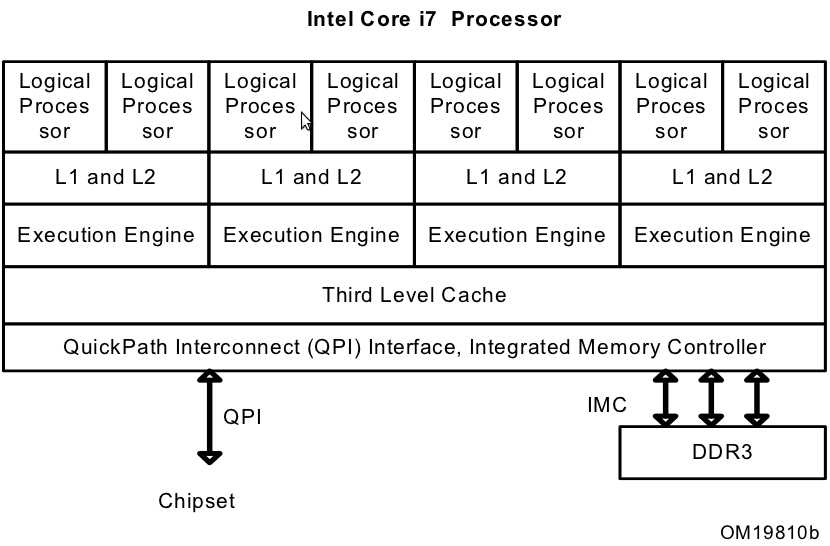
\includegraphics[width=\textwidth]{fig/intel-cache-orga.png}
  \caption{\JWPcpu{} cache organization (taken from \cite{intel2011softdev1})}
  \label{fig:cache-orga}
\end{figure}


%-  general  -----------------------------------------------------------------
\JWlthree{General}
\label{sec:sandy-brige-general}

The most evident characteristics of the \JWPcpu{} are the four cores (on one
chip) and the very uniform distribution of the caches (see figure
\ref{fig:cache-orga}). All caches except for the last-level cache (L3) are
present on each core \cite{fog11}. A short overview over the key features
follows (\cite{intel2011spec}):

\begin{itemize}

\item Number of cores: 4

\item CPU clock speed: \SI{3.4}{\giga\hertz}

\item L1 cache of \SI{64}{\kibi\byte} per core\cite{intel2011softdev1}

\item L2 cache of \SI{256}{\kibi\byte} per core\cite{intel2011softdev1}

\item shared L3 cache of \SI{8}{\mebi\byte}\cite{intel2011softdev1}

\end{itemize}


%-  PMU  -----------------------------------------------------------------------
\JWlthree{Performance Monitoring Unit}
\label{sec:pmu}

The CPU's \emph{Performance Monitoring Unit} (PMU) is present since the
Intel\TReg{} Pentium processor. Using this unit you can monitor several
of the CPU's performance parameters, originally meant for tuning system and
application performance (mostly used by compiler developers)
\cite{intel2011softdev3b}.

In prior work (\cite{bellosa2000benefits,snowdon2010operating,
weissel2002process,kellner03tempcontrol,bertran2010decomposable}) some of these
performance events have proven to be somehow related to the power consumption of
the CPU. As the selection of the events and the degree of their correlation to
energy highly varies between CPUs (or at least CPU microarchitectures) this has
been done again in this work. This time for the Intel\TReg{} Sandy Bridge
microarchitecture and in particular the \JWPcpu{}.

Examining the documentation \cite{intel2011events} approximalely 184 events have
been found available and usable. Because the CPU is only able to count eight
(four in Hyper-threading \cite{wiki:HT} mode) user-programmable performance
events at a time \cite{intel2011softdev1} the most useful events had to be
selected (see chapters \ref{sec:min-events} and \ref{sec:finding-useful-subset}
for a description of  the selection process). In addition to the eight (four)
events, the CPU provides three counters for fixed events, which will be counted
anyway: \JWctr{CPU\_CLK\_UNHALTED.REF\_TSC}, \JWctr{CPU\_CLK\_UNHALTED.THREAD}
and \JWctr{INST\_RETIRED.ANY}.

The selection, configuration and usage of these performance event counters is
done via special \emph{model specific registers} (MSRs), see
\cite{intel2011softdev3b} for the documentation. In this work a more high-level
approach via the \texttt{perf\_event}-API of newer Linux Kernels (some
documentation available at \cite{weaver2011perfevents}) and \JWtool{libpfm4}
(see chapter \ref{sec:standard-software}) has been used.


%-  architectural differences  -------------------------------------------------
\JWlthree{Architectural Differences between Sandy Bridge and Older Architectures}

The Intel\TReg{} \emph{Sandy Bridge} microarchitecture is a further development
of the Core and Nehalem architectures \cite{fog11}. Among other simplifications
of the branch prediction unit, the special loop predictor has been decontinued
presumably to reduce the overall pipeline length and to minimize the
misprediction penalties \cite{fog11}. For speed-improvements a micro-operation
($\mu$op) cache and macro-operation fusion have been introduced \cite{fog11}.


\JWlone{Design}
\label{sec:design}


%#  BIG PICTURE  ###############################################################
\JWltwo{Big Picture of the Setup}
\label{sec:big-pic}

\begin{figure}
  \centering
    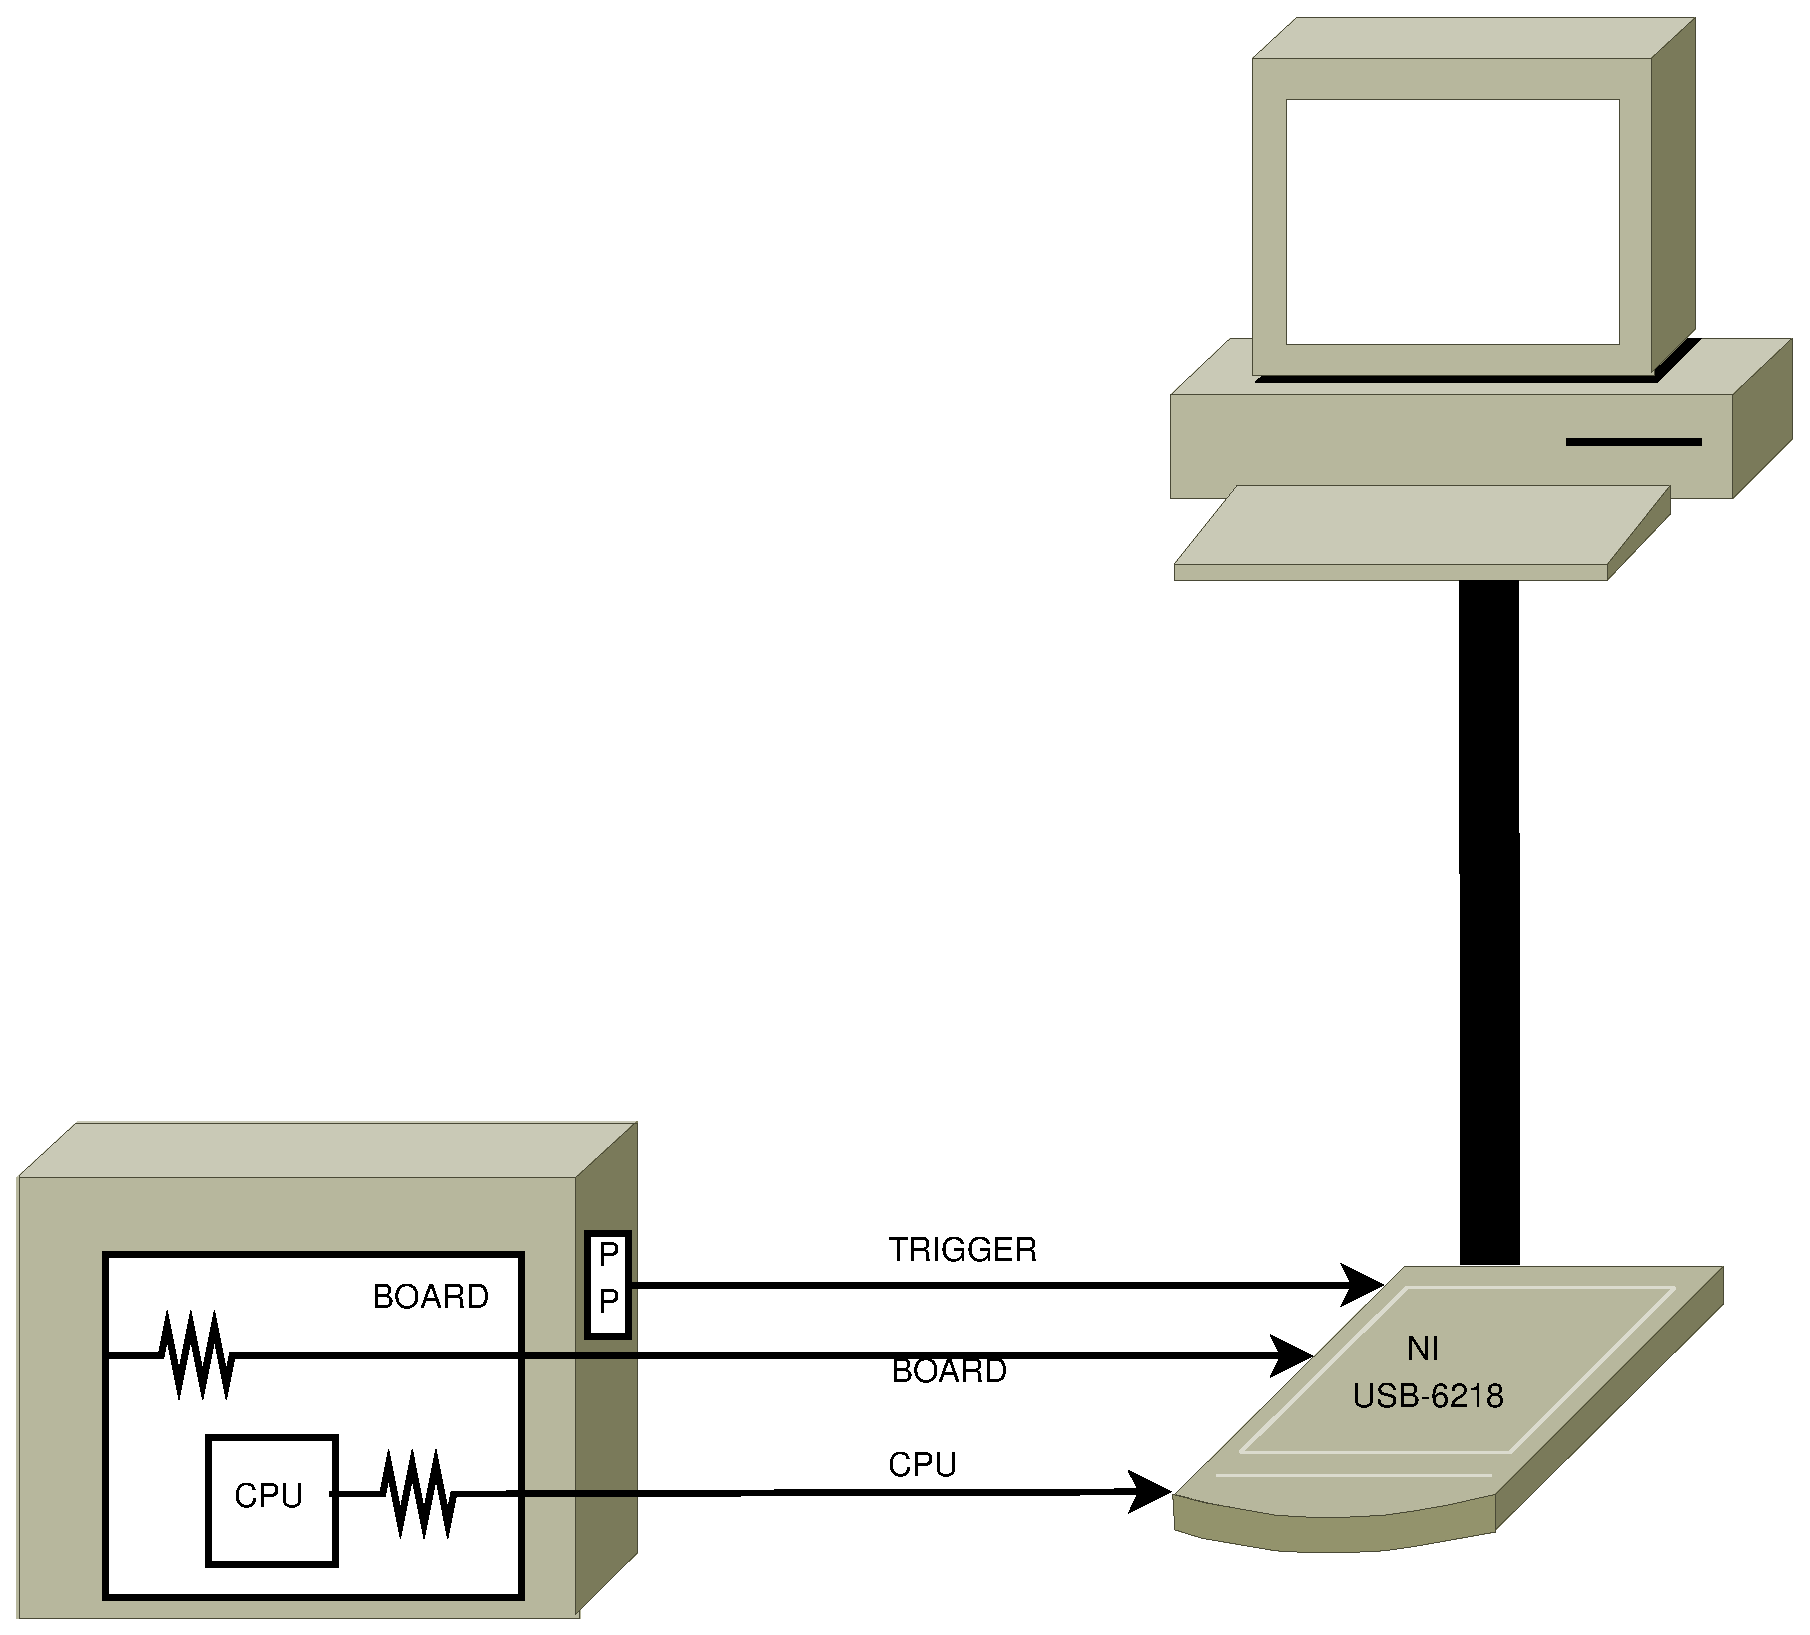
\includegraphics[width=\textwidth]{fig/measuring-overview.eps}
  \caption{Measuring setup overview}
  \label{fig:overview}
\end{figure}

As figure \ref{fig:overview} illustrates an additional workstation---the
\emph{Examining Workstation (EW)}---has been used while evolving this thesis.
The \emph{System under Test (SuT)} counts the CPU's performance events itself
and the EW records the energy consumption using a measuring device in the
meantime. These two data sets have thereafter been used to build up the energy
model.


%#  MEASURING SETUP IN DETAIL  #################################################
\JWltwo{Measuring Setup in Detail}
\label{sec:measuring-setup}

To fit the energy model later, the current flows of the CPU and the
motherboard's \SI{12}{\volt} supply have to be measured. Using four--terminal
sensing \cite{wiki:FTS} voltage drops across the sensing resistor are
measured to deduce the current flow. The motherboard's \SI{12}{\volt} current
flow has been measured in this thesis because it was unclear if the CPU is
entirely fed by its own \SI{12}{\volt} power supply.

Because the SuT and the EW (see figure \ref{fig:overview}) have to agree about
the examination (time) interval a trigger wire is used. It is realized as a
simple analog signal using the parallel port's \emph{high} and \emph{low}
voltages.

This can be summed up to measure three potential differences. Since the
measuring device (chapter \ref{sec:measuring-device}) provides up to eight
differential, analog input channels this seems easy at first. Unfortunately,
two caveats apply: On the one hand according to the user's manual
\cite{NIManual2009} the best measuring accuracy can be achieved in range of
\SI{-200}{\milli\volt} and \SI{200}{\milli\volt}. On the other hand the overall
potential differences may not exceed $\pm$\SI{10.4}{\volt} \cite{NISpec2009}.

\begin{figure}
  \centering
    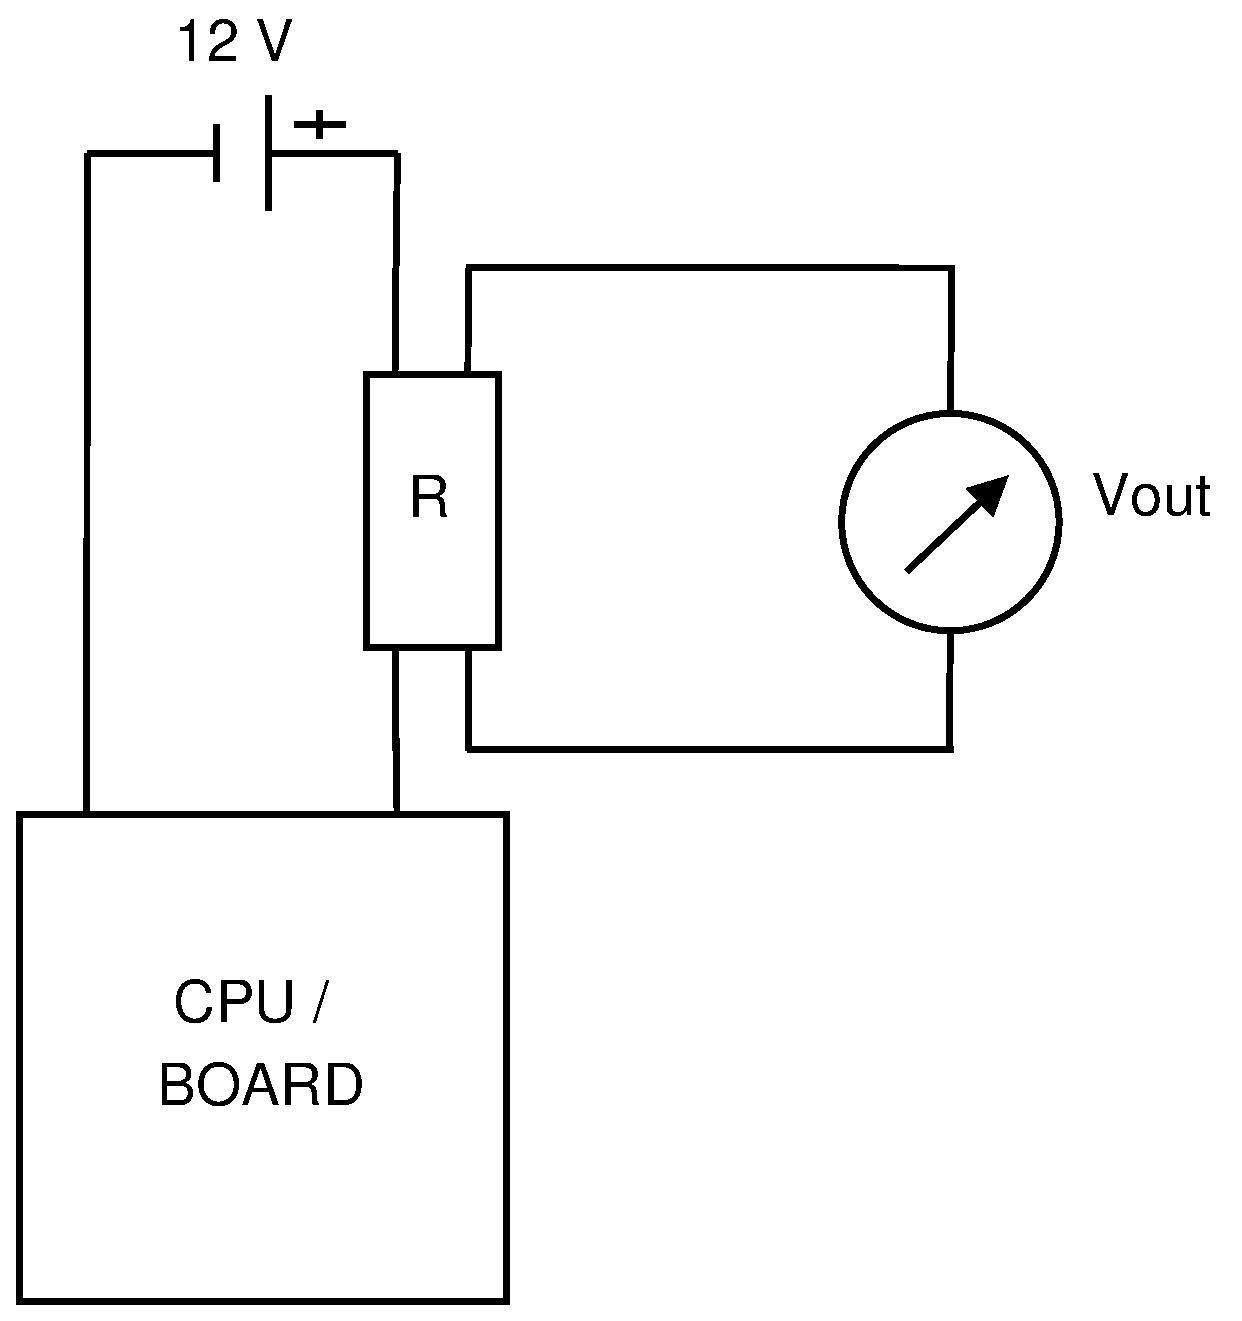
\includegraphics[width=0.5\textwidth]{fig/measuring-circuit.eps}
  \caption{Measuring circuit for CPU (R=\SI{10}{\milli\ohm}) and BOARD
(R=\SI{5}{\milli\ohm})}
  \label{fig:circuit}
\end{figure}

\begin{figure}
  \centering
    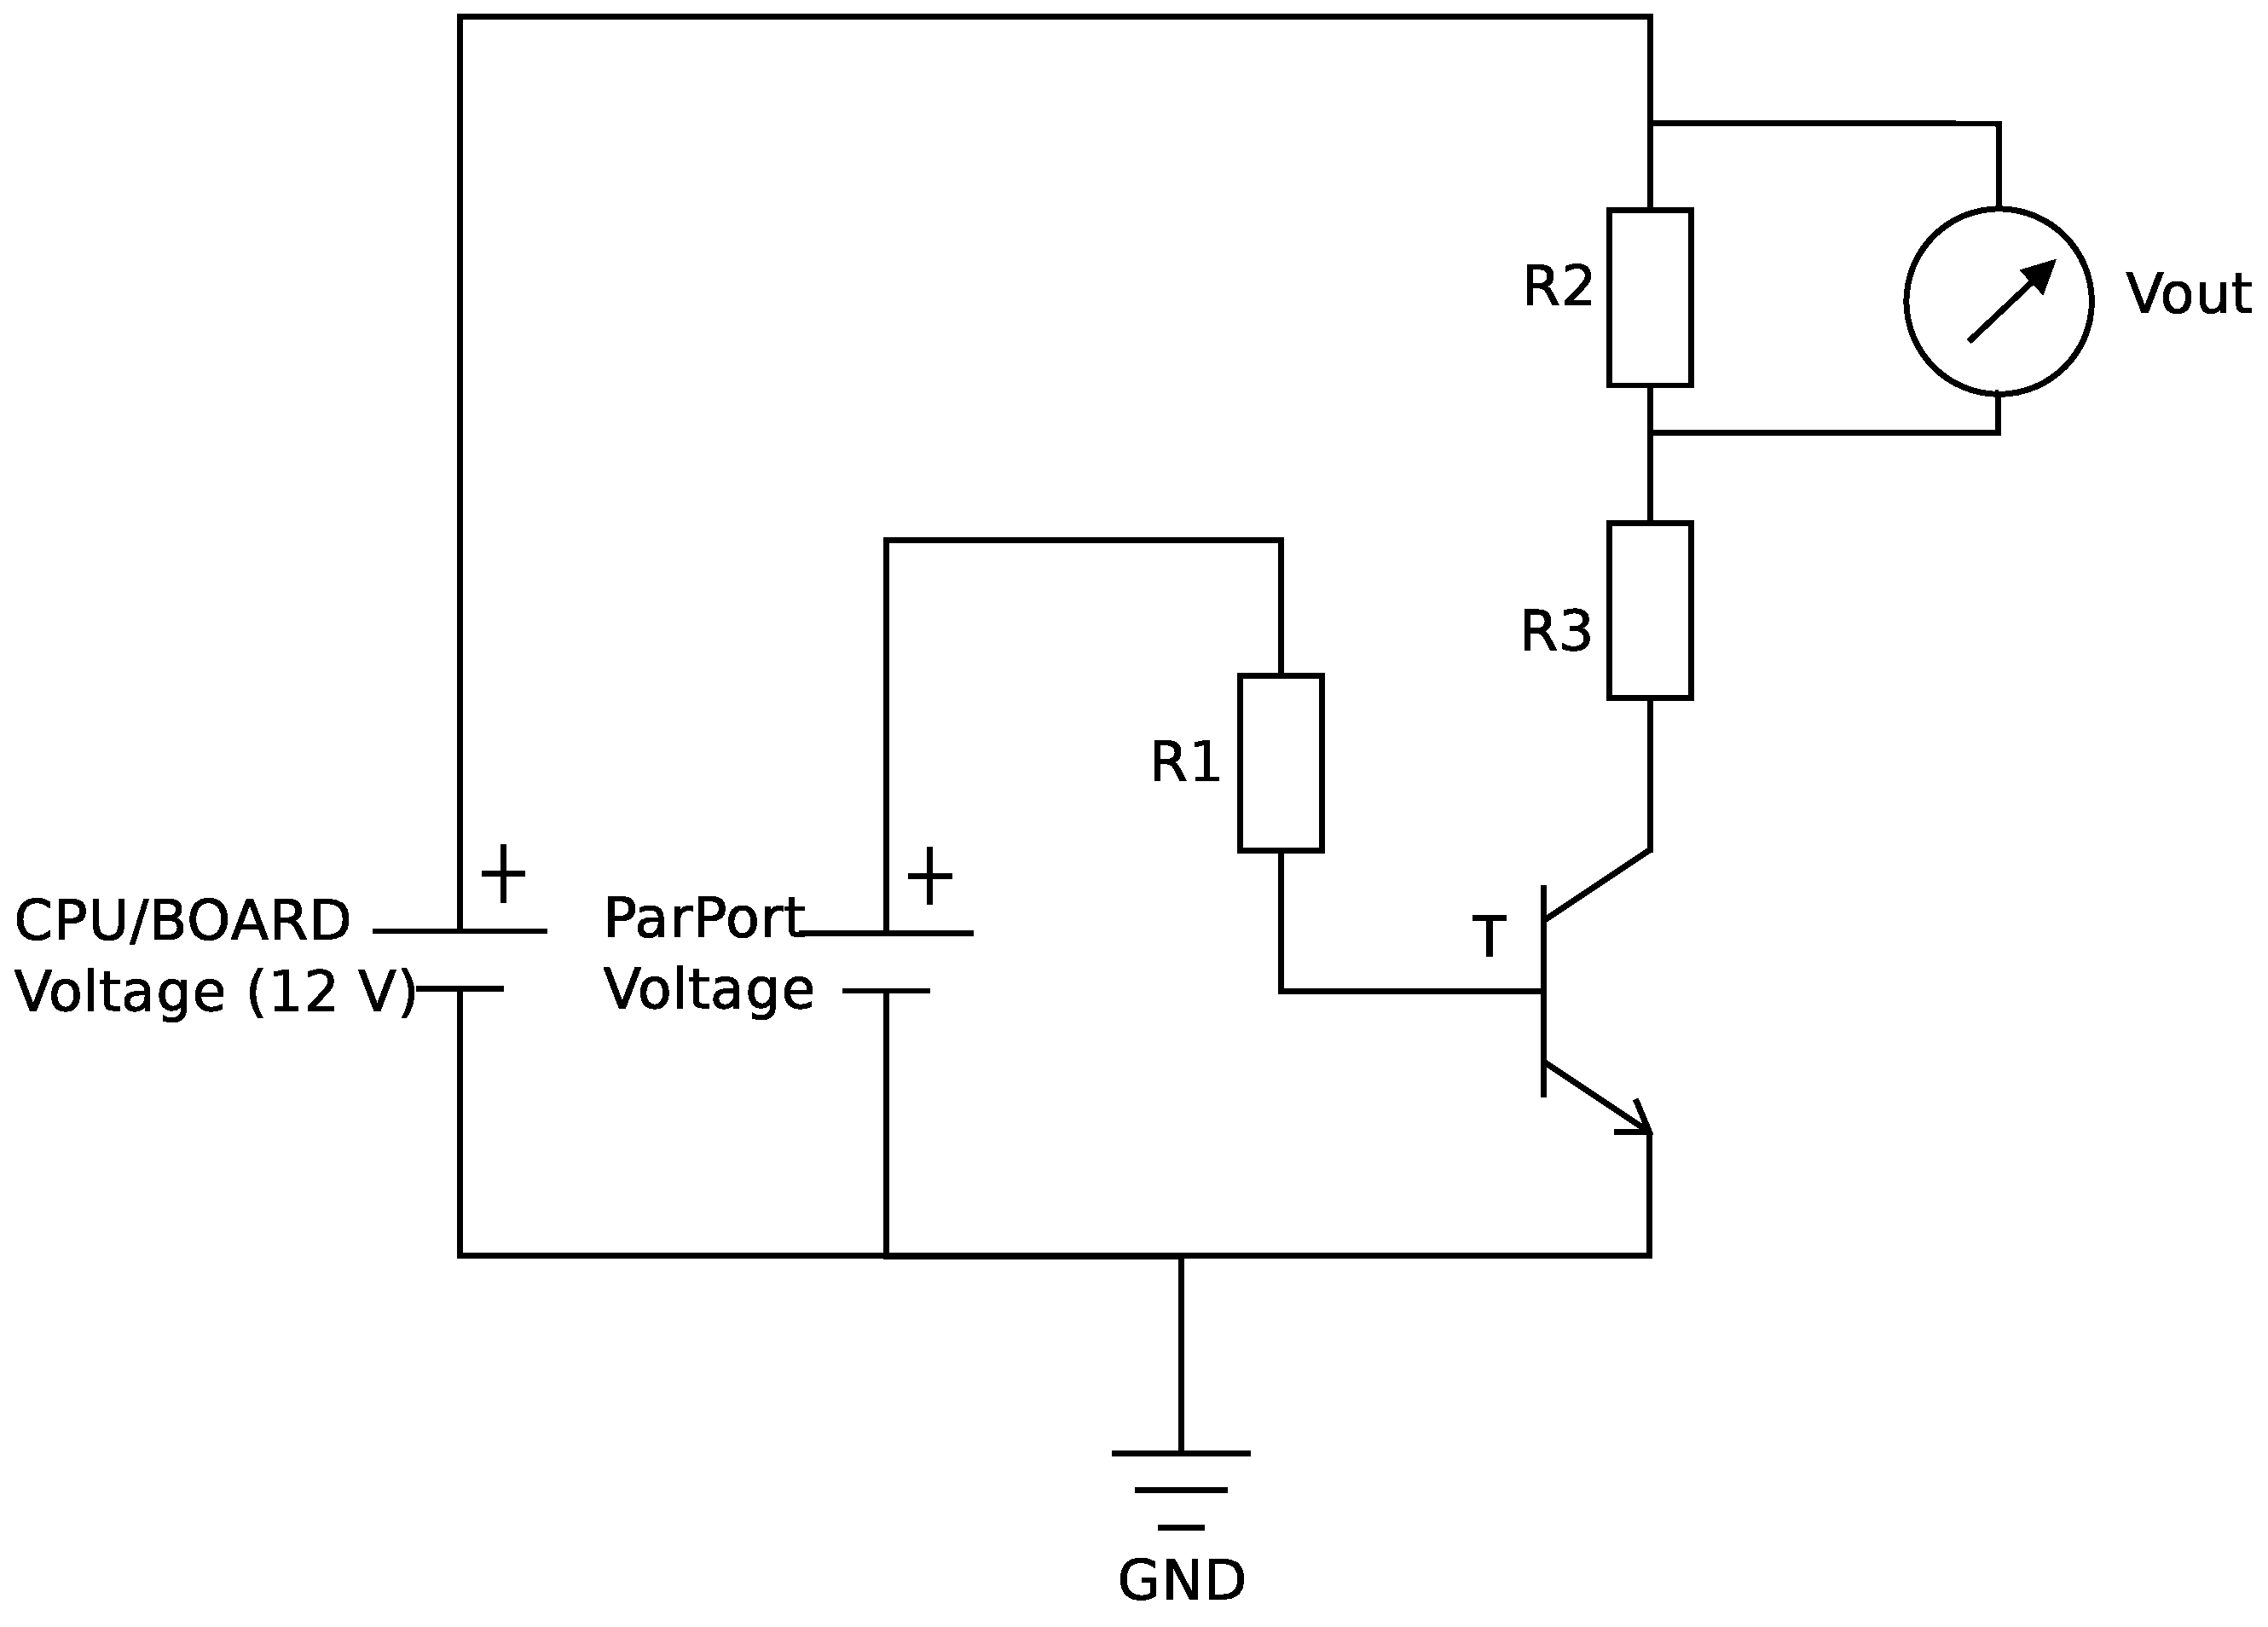
\includegraphics[width=\textwidth]{fig/potential-equalizer.eps}
  \caption{Potential equalizer}
  \label{fig:potential-equalizer}
\end{figure}

Choosing adequate sensing resistors for the \JWchan{CPU} (R =
\SI{10}{\milli\ohm}) and \JWchan{BOARD} (R = \SI{5}{\milli\ohm}) channels (see
figure \ref{fig:circuit}) worked out well. The parallel port trigger wire has
been a problem at first, though. The parallel port has a potential difference
range of more than \SI{200}{\milli\volt} and our test machine's port had a very
different potential level than the \JWchan{CPU} and \JWchan{BOARD} channels,
exceeding the allowed range of $\pm$\SI{10.4}{\volt}.  The potential equalizer
illustrated in figure \ref{fig:potential-equalizer} solves both problems.

Finally, three differential channels \JWchan{CPU}, \JWchan{BOARD}
(\SI{12}{\volt} supply only!) and \JWchan{TRIGGER} in the range of
$\pm$\SI{200}{\milli\volt} and alike potential levels can be connected to the
measuring device. The performance events get counted on the SuT itself which
controls the trigger wire, too: The trigger is set to \emph{On} directly before
executing the program to examine and is set to \emph{Off} promptly after its
termination. To safely register all CPU energy consumption peaks, a high
sampling rate of \SI{50}{\kilo\samples\per\second} is chosen. An exemplary
plot of an examination can be found in figure \ref{fig:cpu-power-trig}.

\begin{figure}
  \centering
    \includegraphics[width=\textwidth]{fig/cpu-power-trig.eps}
  \caption{Sample examination}
  \label{fig:cpu-power-trig}
\end{figure}


%-  measuring device  ----------------------------------------------------------
\JWlthree{Measuring Device}
\label{sec:measuring-device}

For measuring the voltage drops \JWPLni{} from
\JWenterprise{http://www.ni.com}{National Instruments} (shown in figure
\ref{fig:ni}) was chosen because it supports high sampling rates of up to 250000
samples per second (\SI{250}{\kilo\samples\per\second}) and is very accurate
(accuracy $< \SI{2.69}{\milli\volt}$)\cite{NISpec2009}.

\begin{figure}
  \centering
    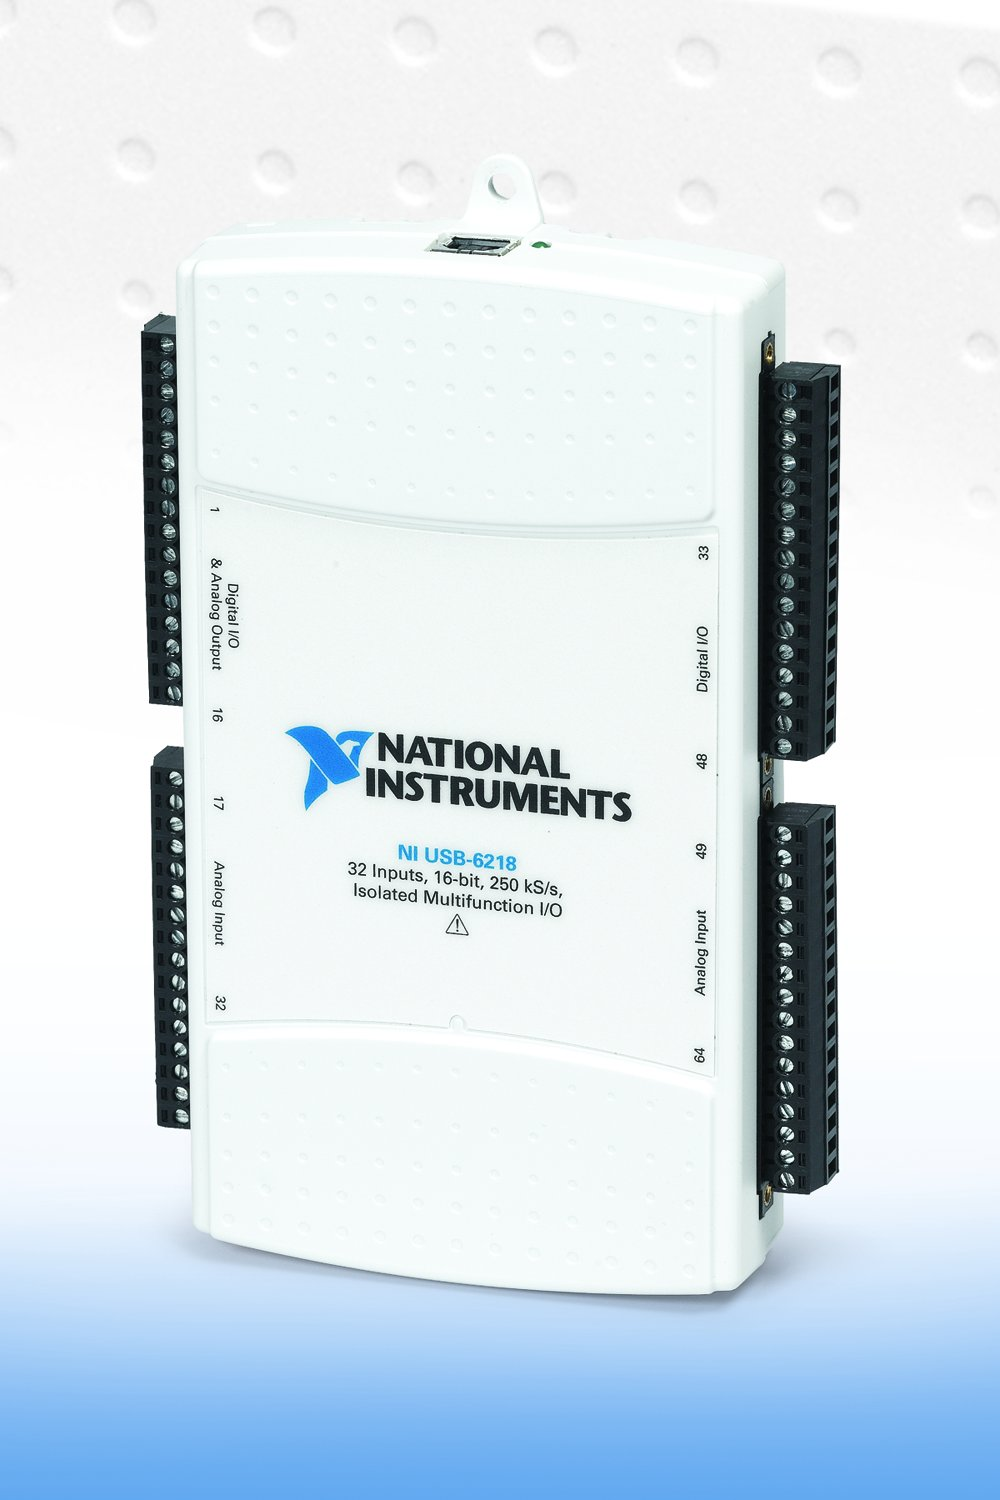
\includegraphics[width=0.5\textwidth]{fig/NI-USB-6218.jpg}
  \caption{\JWPni{} (picture from \JWlink{http://www.pressebox.de/pressemeldungen/national-instruments-germany-gmbh/boxid/75241})}
  \label{fig:ni}
\end{figure}


%#  CALCULATION OF THE ELECTRICAL WORK  ########################################
\JWltwo{Calculation of the Electrical Work}
\label{sec:calc-work}

From elementary physics:

\begin{eqnarray}
     U = R * I \iff I = \frac{U}{R} \\
     P = U * I
\end{eqnarray}

So, the current flow is calculatable from the volatage drops across the
measuring resistor ($U_R$). Accordingly, the instantaneous power can be
calculated as:

\begin{eqnarray}
P    & = & U * I \\
     & = & U * \frac{U_R}{R} \\
P(t) & = & \frac{12V * U_R}{R}
\end{eqnarray}

Hence, integrating will result in the electrical work

\begin{equation}
  W = \int P(t)dt.
\end{equation}


%#  ENERGY MODEL  ##############################################################
\JWltwo{Energy Model}
\label{sec:model}

The following chapters will define the term \emph{energy model} along with  the
formal methods suggested to build such a model.


%-  the model's properties  ----------------------------------------------------
\JWlthree{Properties}
\label{sec:model-properties}

In this work, an energy model is considered as a linear function. A system with
$n_c$ cores that is able to monitor $n_e$ performance events per core
simultaneously is described. Additionally to the per--core event counters, $n_g$
global event counters make the model up. In the formal description (see chapter
\ref{sec:towards-the-model} for the practical implementation) we assume four
functions providing the actual values:

\begin{itemize}

\item $c_g(i, t_0, t_e) \in \mathbb{N}^{\{1, \ldots, n_e\} \times
\mathbb{R}_{\geq 0} \times \mathbb{R}_{\geq 0}}$, the global event $i$'s count
in the time interval $(t_0, t_e)$

\item $c_e(j, k, t_0, t_e) \in \mathbb{N}^{\{1, \ldots, n_c\} \times
\{1, \ldots, n_g\} \times \mathbb{R}_{\geq 0} \times \mathbb{R}_{\geq 0}}$, the
performance event $k$'s count on core $j$ in the interval $(t_0, t_e)$

\item $w_g(i) \in \mathbb{R}^{\{1, \ldots, n_g\}}$, the global event $i$'s
energy weight in \si{\joule}

\item $w_e(j, k) \in \mathbb{R}^{\{1, \ldots, n_c\} \times \{1, \ldots, n_g\}}$,
the weight of performance event $k$ in \si{\joule} on core $j$

\end{itemize}

Though, an energy model equates to a linear function. The function's value is
the electrical work performed between two instants of time $t_0$ and $t_e$:

\begin{equation}
W(t_0, t_e) = \sum\limits_{i=1}^{n_g} c_g(i, t_0, t_e) w_g(i) +
\sum\limits_{j=1}^{n_c} \sum\limits_{k=1}^{n_e} c_e(j, k, t_0, t_e) w_e(j, k)
\end{equation}

The functions $c_e$ and $c_g$ contain the system's life data whereas the energy
weight functions $w_e$ and $w_c$ can be calculated a priori as done in this
work. Obviously, the selection of the events and their respective weights highly
depend on the type of microprocessor. To calculate the electrical power the
system consumes, one typically chooses an arbitrary frequency $T$ and sets the
variables $t_0$ and $t_e$ accordingly ($t_0 = ?$, $t_e = t_0 + \frac{1}{T}$).
The instantaneous power of the instant $t$ (of length $\frac{1}{T}$) is then
calculated as:

\begin{eqnarray}
P(t) & = & \frac{W(t - \frac{1}{T}, t)}{\frac{1}{T}} \\
     & = & \frac{\sum\limits_{i=1}^{n_g} c_g(i, t - \frac{1}{T}, t) w_g(i) +
                 \sum\limits_{j=1}^{n_c}
                 \sum\limits_{k=1}^{n_e} c_e(j, k, t - \frac{1}{T}, t) w_e(j, k)
                }{\frac{1}{T}}
\end{eqnarray}


%-  finding the energy weights  ------------------------------------------------
\JWlthree{Finding the Energy Weights}
\label{sec:finding-weights}

Having seen what exactly constitutes an energy model (chapter
\ref{sec:model-properties}), it is crucial to find a small and significant set
of performance events and appropriate energy weights. This chapter will focus on
how to find the weights, a seperate chapter (\ref{sec:min-events}) describes the
miniaturization of the event set. To find reasonable energy weights, test
program execution (also called benchmark) observations have to be recorded and
evaluated. Of each test program run record, the following data is needed later:

\begin{itemize}

\item $b$, the point of time the run began

\item $e$, the point of time the run ended

\item The $n_g$ values of the functions $c_g(1 \cdots n_g, b, e)$

\item The $n_c * n_e$ values of the functions
$c_e(1 \cdots n_c, 1 \cdots n_e, b, e)$

\item The electrical work $j$ the system performed between $b$ and $e$

\end{itemize}

Since the fitting of the energy weights needs a larger data set, a matrix
representation is appropriate. So, $n_o$ observations in the non--overlapping
time intervals $(b_{1 \cdots n_o}, e_{1 \cdots n_o})$ lead to:

\begin{itemize}

\item $b_{1 \cdots n_o}$, the points of time the runs began

\item $e_{1 \cdots n_o}$, the points of time the runs ended

\item The matrix $Cg$ containing the global counter values (see equation
\ref{eqn:cg})

\item The matrix $Ce$, containing the performance event counter values (see
equation \ref{eqn:cc})

\item The vector $j = <j_1, \cdots, j_{n_o}>$, containing the electrical works
performed

\end{itemize}

\begin{eqnarray}
%% Cg
\label{eqn:cg}
& Cg & \in \mathbb{N}^{n_o \times n_g} \\
& Cg & =
\begin{pmatrix}
c_g(1, b_1, e_1)         & \cdots & c_g(n_g, b_1, e_1)        \\
\vdots                   & \ddots & \vdots                    \\
c_g(1, b_{n_o}, e_{n_o}) & \cdots & c_g(n_g, b_{n_o}, e_{n_o})
\end{pmatrix} \\
%% Ce
\label{eqn:cc}
& Ce & \in \mathbb{N}^{n_o \times n_cn_e } \\
& Ce & =
\begin{pmatrix}
c_e(1, 1, b_1, e_1)         & \cdots & c_e(n_c, n_e, b_1, e_1)         \\
\vdots                      & \cdots & \vdots                          \\
c_e(1, 1, b_{n_o}, e_{n_o}) & \cdots & c_e(n_c, n_e, b_{n_o}, e_{n_o})
\end{pmatrix}
\end{eqnarray}

Using a linear regression (of eqation \ref{eqn:lin-reg}), suitable energy
weight vectors $w_c$ and $w_g$ may be found. The goal is to minimize the error
term, i.\,e.\ $\sum\epsilon^2$ is small as possible.

\begin{equation}
\label{eqn:lin-reg}
j = C w + \epsilon
\end{equation}

\begin{eqnarray*}
%% j
j & = &
\begin{pmatrix}
j_1 \\
\vdots \\
j_{n_o}
\end{pmatrix} \\
%% C
C & = & \big( Cg \arrowvert Ce \big) \in \mathbb{N}^{n_o \times n_g+n_cn_e} \\
& = &
\begin{pmatrix}
Cg_{1,1}   & \cdots & Cg_{1,n_g}   & Ce{1,1}   & \cdots & Ce{1,n_cn_e} \\
\vdots     & \ddots & \vdots       & \vdots    & \ddots & \vdots       \\
Cg_{n_o,1} & \cdots & Cg_{n_o,n_g} & Ce{n_o,1} & \cdots & Ce{n_o,n_cn_e} \\
\end{pmatrix} \\
%% w
w & = &
\begin{pmatrix}
w_g(1) \\
\vdots \\
w_g(n_g) \\
w_e(1, 1) \\
\vdots \\
w_e(n_c, n_e)
\end{pmatrix} \\
\end{eqnarray*}


%-  minimizing the counter set  ------------------------------------------------
\JWlthree{Minimizing the Set of Performance Events}
\label{sec:min-events}

It is not practical to take into account all events the microprocessor is aware
of. Today's processors offer a lot more events then they can count
simultaneously \cite{intel2011softdev1}. The functions and matrices names of the
previous chapter (\ref{sec:finding-weights}) also apply here. The single
exception is that this chapter only focusses on the CPU's performance events.
The global events are not taken into account here because they are
pseudo--events not obtained by the limited PMU. The approach to find a subset of
$n_e$ events (of $e_{max}$ available) used in this work can be summed up to:

\begin{enumerate}

\item Generation of the matrix of performance event counters $Ce$ and
the corresponding vector of electrical works $j$

\item Obtaining $Ce_{final}$ containing the $n_e$ most correlating columns of
$Ce$ that will form the energy model's performance events

\end{enumerate}

Thereafter, the performance events the model finally uses are found. The next
step is to find the final energy weights as in the previous chapter
(\ref{sec:finding-weights}).


\JWlfour{Step 1: Generating $Ce$ and $j$}

\begin{enumerate}[(a)]

\item Choose $p$ test programs which use the CPU differently. The test
programs have to be independent from external events. We consider subsequent
runs of a test program as equal.

\item Divide the $e_{max}$ available events in $g$ disjoint, non--empty sets
$E_{1..g}$ of size up to $n_e$.

\item For each set $E_{1..g}$, run all the $p$ test programs and record the
electrical work performed and the event counters of the set's events.

\item The electrical work of each of the runs of a test program should be
roughly equal. If they differ a lot, there is either a dependency on external
events in the benchmark or the machine is otherwisely stressed. In the former
case the test program selection should be improved, in the latter the affected
test runs have to be repeated.

\item Folding all the results leads to a vector $j_{1..p}$ containing the
electrical work a run of each of the test programs performed. Additionally, a
matrix $Ce$ (as in chapter \ref{sec:finding-weights}) arises, containing each
event counter's value for a run of each of the test programs.

\end{enumerate}

\JWlfour{Step 2: Deriving $Ce_{final}$ from $Ce$}

\begin{enumerate}[(a)]

\item Eliminate duplicate columns in $Ce$

\item Eliminate columns that contain only zeroes in $Ce$

\item Eliminate linear dependent columns in $Ce$

\item Generate all column combinations of size $n_e$ (without repetition) of the
remaining columns in $Ce$, generate energetical weights (as in chapter
\ref{sec:finding-weights})

\item $Ce_{final}$ is the combination with the smallest error term
($\sum\epsilon^2$)

\end{enumerate}

% vim: set spell spelllang=en_us fileencoding=utf8 : syntax spell toplevel :


\JWlone{Implementation}

%#  DATA FORMATS  ##############################################################
\JWltwo{Data Formats}
\label{sec:data-formats}

In this section the in memory and on disk data formats will be presented. The
basic protocol is \JWTprotobuf.

%-  voltage drop data point files  ---------------------------------------------
\JWlthree{Voltage Drop Data Point Files}
\label{sec:datapoint-files}


%-  performance counter files  -------------------------------------------------
\JWlthree{Counter Files}
\label{sec:counter-files}


%#  TOOLS  #####################################################################
\JWltwo{Tools}
\label{sec:tools}

Since the building of a reasonable energy model is not an easy task, numerous
tools have been used. Most of the tools were developed specifically for the
purpose of this study thesis. All of them are open-sourced and available on
\JWnamedlink{https://github.com/weissi/studienarbeit}{GitHub}.

In this chapter, we will give an overview of the software used, both standard
software and tools developed specifically to be able to write this paper.


%-  standard software  ---------------------------------------------------------
\JWlthree{Standard Software}
\label{sec:standard-software}

\begin{itemize}

\item \JWTprotobuf for saving and loading of all kinds of data

\item \JWnamedlink{http://www.r-project.org/}{R} for statistical computations

\item \JWnamedlink{http://cran.r-project.org/web/packages/leaps/}{leaps package}
      , a R library for regression subset selection (to minimize the set of
      available performance counters)

\item \JWnamedlink{http://stat.ethz.ch/R-manual/R-devel/library/stats/html/lm.html}
      {lm library}, a R library used to fit linear models

\item \JWnamedlink{http://kernel.org}{Linux Kernel}

\item \JWnamedlink{http://gnu.org}{numerous GNU tools}

\end{itemize}


%-  special developments  ------------------------------------------------------
\JWlthree{Special Developments}
\label{sec:special-developments}


\JWlfour{\JWTlibdp}

\JWTlibdp is responsible for loading and saving the measured data points from
and to the \JWTprotobuf files. It's API is straight forward and it is able to
handle very big files. The API can be found in
\JWpath{libdatapoints/datapoints.h}.


\JWlfour{\JWTfcw}

\JWTfcw can calculate the electrical work from data points files very quickly.
As explained in section \ref{sec:calc-work} it integrates to electrical power.
But since we obtain discrete data by sampling (see section
\ref{sec:measuring-setup}) the integration can be done quite fast:

\JWtodo{integral P = sum P * diff}

A typical call to \JWTfcw looks like

\begin{lstlisting}[style=Shell]
fastcalcwork captured-17:15:00.dpts CPU 0.01 TRIGGER
\end{lstlisting}

Using the command line above, \JWTfcw will calculate the electrical work with a
measuring resistor of \SI{0.01}{\ohm}. The measured data points will be taken
from column \texttt{CPU}, the analog trigger's (see section
\ref{sec:measuring-setup}) value from \texttt{TRIGGER}.


\JWlfour{\JWTdc}

\JWTdc is the tool for retrieving the performance counter's values on the target
machine. Giving it a set of performance counters and a command to execute, it
will record the counters while the command is running. It always works
system-wide and saves values by counter and by CPU enabled.

A working example:

\begin{lstlisting}[style=Shell]
dumpcounters -e CPU_CLK_UNHALTED,INST_RETIRED -r ls
\end{lstlisting}

The exact data format is documented in \JWpath{protos/perf-counters.proto}.

\JWlfour{\JWTde}

\JWTde exports data point files (see section \ref{sec:datapoint-files}) to a
format \JWTR can easily use.

\JWtodo{bib ref to R table format}.

\JWlfour{\JWTdd}

\JWlfour{\JWTcbs suite}

\JWlfour{\JWTbsle}

\JWlfour{high-level scripts}


%#  METHODS OF ANALYSIS  #######################################################
\JWltwo{Methods of Analysis}
\label{sec:methods-of-analysis}

In this section the mathematical and formal methods to find a good subset of
events and their coefficients is presented.


%#  TOWARD THE ENERGY MODEL  ###################################################
\JWltwo{Toward the Energy Model}
\label{sec:towards-the-model}

In this chapter a description of the steps toward the final energy model(s) is
given.


%-  BENCHMARKS  ----------------------------------------------------------------
\JWlthree{The set of Benchmarks}
\label{sec:benchmarks}

How and which benchmarks did I choose?


%-  SUBSET OF USEFUL COUNTERS  -------------------------------------------------
\JWlthree{Finding a useful Subset of Events}

\begin{itemize}

\item 1 CPU, all events, rotational

\item 1 CPU enabled, chosen events

\item 2 CPUs enabled, chosen events

\item 3 CPUs enabled, chosed events

\item 4 CPUs enabled, chosed events

\end{itemize}



% vim: set spell spelllang=en_us fileencoding=utf8 :


\JWlone{Evaluation}
\label{sec:evaluation}

What does it mean?

%%%%%%%%%%  schrieblesque
%%%%%%%%%%
%%%%%%%%%%  SCHRIEBLESQUE


% #  ERROR OF ESTIMATION  ######################################################
\JWltwo{Error of Estimation}
\label{sec:error}

Presentation of measured and estimated work. Plus errors.


% #  COMPARISON TO SIMPLE TIME BASED MODEL  ####################################
\JWltwo{Comparison to a simple time based Model}
\label{sec:time-based}

This chapter features a comparison of the gained energy model to a simple
time-(only-)based one.


% #  OVERHEAD IMPLEMENTATION  ##################################################
\JWltwo{Overhead of this Implementation}
\label{sec:overhead}

How many CPU clock cycles do I waste for the accounting the performance
counters.


% #  VARIATION BETWEEN RUNS  ###################################################
\JWltwo{Variation of Results between Runs}
\label{sec:variation}

Are there variations of the results between the runs?


\JWlone{Conclusion}

As of our knowledge the energy model presented in this thesis is the first
performance event counter based for the Intel\TReg{} Sandy Bridge
microarchitecture. Over the above it is the first for CPUs with more than two
cores. The evaluation results prove the general concept is also applicable to
today's and tomorrow's multi--core CPUs.

The software developed along with this thesis provides a convenient and freely
available way to build energy models in the future.


% #  PROBLEMS  #################################################################
\JWltwo{Problems and Outlook}
\label{sec:problems}

Even though the resulting energy model already proved its efficiency and
necessity, there is room for further improvements. On the one hand for the model
itself, on the other hand for the process of building energy models for new
target architectures. First, the restrictions mentioned in chapter
\ref{sec:restrictions} should be eliminated. To improve the practical usefulness
real multi--threading programs should be better kept in mind. The challenge with
threads is that shared memory regions get accessed on the same time. This will
probably attract interest on other or additional performance events which are
not well covered here. The latter also shows the need to develop a convenient
event selection process. Supplementary, the upcoming many--core architectures
with $\gg 4$ cores could become challenging.

% vim: set spell spelllang=en_us fileencoding=utf8 : syntax spell toplevel :


\backmatter
\addcontentsline{toc}{chapter}{Bibliography}
\bibliography{bibliography}
\appendix
\appendixpage
\addappheadtotoc

\renewcommand\thesection{\Alph{section}}
\chapter{Appendix}

\JWlappendix{Performance Event Selection and Description}
\label{appendix:chosen-events}

This section lists all the performance events which form the energy model
presented in this work. The descriptive texts are all taken from
\cite{intel2011events}.

\begin{itemize}

\item \JWctr{CPU\_\-CLK\_\-UNHALTED}
\begin{quotation}
This is an architectural event that counts the number of thread cycles while the
thread is not in a halt state. The thread enters the halt state when it is
running the HLT instruction. The core frequency may change from time to time due
to power or thermal throttling. For this reason, this event may have a changing
ratio with regards to wall clock time.
\end{quotation}

\item \JWctr{INST\_\-RETIRED}
\begin{quotation}

This event counts the number of instructions retired from execution. For
instructions that consist of multiple micro-ops, this event counts the
retirement of the last micro-op of the instruction. Counting continues during
hardware interrupts, traps, and inside interrupt handlers. Notes:
\JWctr{INST\_\-RETIRED.\-ANY} is counted by a designated fixed counter, leaving
the four (eight when Hyper\-threading is disabled) programmable counters
available for other events. \JWctr{INST\_\-RE\-TI\-RED.\-ANY\_\-P} is counted by
a programmable counter and it is an architectural performance event. Counting:
Faulting executions of GETSEC / VM entry / VM Exit / MWait will not count as
retired instructions.

\end{quotation}

\item \JWctr{BR\_\-INST\_\-RETIRED:FAR\_\-BRANCH}
\begin{quotation}
This is a non-precise version (that is, does not use PEBS) of the event that
counts far branch instructions retired.
\end{quotation}

\item \JWctr{DSB2MITE\_\-SWITCHES}
\begin{quotation}
This event counts the number of the Decode Stream Buffer (DSB)-\-to-\-MITE
switches including all misses because of missing Decode Stream Buffer (DSB)
cache and u-arch forced misses. Note: Invoking MITE requires two or three cycles
delay.
\end{quotation}

\item \JWctr{DSB\_\-FILL:ALL\_\-CANCEL}
\begin{quotation}
This event counts the number of times when a valid Decode Stream Buffer (DSB)
fill has been actually cancelled not because of exceeding the way limit.
Cancelling Decode Stream Buffer (DSB) fill may also result, for example, from
Decode Stream Buffer Queue (DSBQ) snoop hits. This is because the Decode Stream
Buffer (DSB) full hit is guaranteed to delivery from Decode Stream Buffer (DSB).
In the B step a four-bit counter will count the number of cancel operations and
will reverse the priority upon look ing up the same set.
\end{quotation}

\item \JWctr{ILD\_\-STALL:IQ\_\-FULL}
\begin{quotation}
This event counts stall cycles when instructions cannot be written because IQ is
full. Note: If there is no Resource Allocation Table (RAT) stalls, it indicates
the decoders issue.
\end{quotation}

\item \JWctr{L2\_\-RQSTS:PF\_\-HIT}
\begin{quotation}
This event counts the number of requests from the L2 hardware prefetchers that
hit L2 cache. LLC prefetch new types
\end{quotation}

\item \JWctr{LD\_\-BLOCKS:ALL\_\-BLOCK}
\begin{quotation}
Number of cases where any load ends up with a valid block-code written to the
load buffer (including blocks due to Memory Order Buffer (MOB), Data Cache Unit
(DCU), TLB, but load has no DCU miss)
\end{quotation}

\item \JWctr{LD\_\-BLOCKS:DATA\_\-UNKNOWN}
\begin{quotation}
This event counts the number of load operations delayed due to store buffer
blocks, preceding store operations with known addresses but unknown data.
Counting happens according to the final blocking codes. This does not include
inline wakeups.
\end{quotation}

\item \JWctr{UOPS\_\-DISPATCHED:STALL\_\-CYCLES}
\begin{quotation}
This event counts cycles during which no uops were dispatched from the
Reservation Station (RS) per thread.
\end{quotation}

\end{itemize}



\JWlappendix{File Formats}

\JWlsubappendix{Data Points File's Format}
\label{sec:fmt:datapoints}
For the definition of the Protocol Buffers used, see appendices
\ref{sec:pb:datapoints} and \ref{sec:pb:generic}. For the definition of the
Protocol Buffer's language see their
\JWnamedlink{http://code.google.com/apis/protocolbuffers/docs/proto.html}{web
site}.

\begin{Verbatim}[baselinestretch=1,fontsize=\scriptsize]
byte 0x03;                            # \
byte 0x01;                            #  THESE BYTES FORM THE FILE
byte 0x86;                            #  FORMAT'S MAGIC BYTES
byte 0x01;                            # /

byte version;                         # THE FORMAT'S VERSION: 0x1

uint32_t header_length;               # LENGTH OF FOLLOWING PROTOCOL BUFFER IN
                                      # BYTES (ENCODING: LITTLE ENDIAN)

<Protocol Buffer type 'MessageData'>  # THE "HEADER" PROTO BUF

REPEATED FOR EVERY CHUNK:
    byte 0x03;                        # \
    byte 0x01;                        #  THESE BYTES FORM THE FILE
    byte 0x86;                        #  CHUNK'S MAGIC BYTES
    byte 0x02;                        # /

    uint32_t message_length;          # LENGTH OF FOLLOWING PROTOCOL BUFFER IN
                                      # BYTES (ENCODING: LITTLE ENDIAN)

    <Protocol Buffer type 'DataSet'>  # THE DATA OF ONE CHUNK
\end{Verbatim}


\JWlsubappendix{Generic Protocol Buffers}
\label{sec:pb:generic}
\begin{verbatim}
message Timestamp {
    required int64 sec = 1;
    required int64 nsec = 2;
}
\end{verbatim}


\JWlsubappendix{Data Points Protocol Buffers}
\label{sec:pb:datapoints}
\begin{verbatim}
import "generic.proto";

message MeasuredData {
    required string shot_id = 1;
    required double sampling_rate = 2;
    required uint32 channel_count = 3;
    required bool has_external_data = 4;
    repeated DataSet inline_data = 5;
    repeated string channel_names = 6; //ordered!
}

message DataSet {
    required Timestamp time = 1;
    repeated DataPoints channel_data = 2;
}

message DataPoints {
    repeated double data_points = 1 [packed=true];
    optional uint32 channel_no = 2;
    optional string channel_name = 3;
}
\end{verbatim}


\JWlsubappendix{Performance Event Counter Protocol Buffers}
\label{sec:pb:counter-files}
\begin{verbatim}
import "generic.proto";

message CounterData {
    required string shot_id = 1;
    required Timestamp start_time = 2;
    required Timestamp stop_time = 3;
    required uint32 cpu_count = 4;
    repeated CounterValue counters = 5;
    optional string benchmark_cmd = 6;
}

message CounterValue {
    required string counter_name = 1;
    repeated uint64 counter_value_per_cpu = 2; //ordered by cpu id
    optional uint64 global_counter_value = 3;
}
\end{verbatim}



\end{document}
% vim: set spell spelllang=en_us fileencoding=utf8 :
